\section{极小值的存在}
\label{sec:func-existence}

不解任何方程，怎样断定一个泛函优化问题有解？这件事比有限维更需要先做，因为后面的最优性条件都以“设$u^\star$是极小点”开头，极小点若不存在，由条件解出的东西就没有意义。

\paragraph{有限维的论证在哪里断开}
第~\ref{chap:optimization}章的论证是：取一个最小化序列，让它通过三关。序列要留得住，极限要合法，比较要能传到极限。在$\mathbb{R}^n$中，有界序列总有收敛子列，第一关由强制性和紧性解决。

无限维中这一步断开了。取$L^2(0,1)$中的函数$e_k(x)=\sqrt2\sin(k\pi x)$，$k=1,2,\ldots$。它们两两正交，长度都是$1$，于是
\[
 \lVert e_j-e_k\rVert_2=\sqrt2\qquad(j\neq k).
\]
这个序列在单位闭球内，任意两项的距离却始终是$\sqrt2$，没有Cauchy子列，也就没有范数收敛的子列。有界闭集不再紧。

\paragraph{换一种看极限的方式}
图~\ref{fig:func-weak-oscillation}(a)的$e_k$越摆越快，但摆动的正负会相互抵消。若固定一个函数$g$，用积分读取$\langle g,e_k\rangle=\int_0^1g\,e_k\,\mathrm{d}x$，(b)中的读数趋于零，而(a)中函数本身的长度不变。逐个读数都收敛到零，整个函数却没有在范数下靠近零。

\begin{BookInlineFigure}
  \centering
  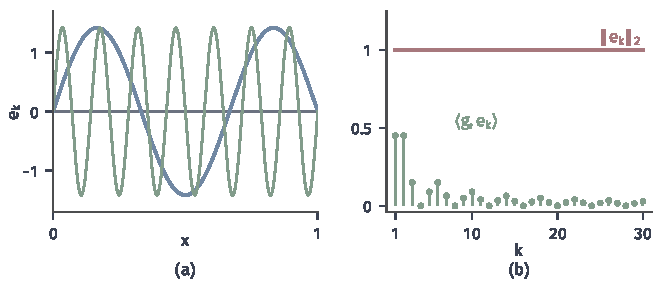
\includegraphics[width=112mm]{figures/05-optimization/08-functional-optimization/matplotlib/func-weak-oscillation/figure.pdf}
  \caption{弱收敛而范数不收敛。(a)$e_k=\sqrt2\sin(k\pi x)$，蓝色$k=3$，绿色$k=14$。(b)红线是$\lVert e_k\rVert_2=1$，绿色竖线是用$g=\mathbf{1}_{[0,1/2]}$读取的$\lvert\langle g,e_k\rangle\rvert$，它随$k$趋于零。}
  \label{fig:func-weak-oscillation}
\end{BookInlineFigure}

这种“每个连续读取都收敛”的收敛称为弱收敛。设$X$是赋范空间，$X^*$是它的对偶空间，即全体连续线性泛函。若对每个$\xi\in X^*$都有$\xi(u^{(k)})\to\xi(u)$，就说$u^{(k)}$弱收敛到$u$，记作$u^{(k)}\rightharpoonup u$。在Hilbert空间中，这就是对每个$g$都有$\langle g,u^{(k)}\rangle\to\langle g,u\rangle$。

弱收敛正好补上第一关。我们使用两条结论。若$X$是反射空间，则每个有界序列都有弱收敛的子列；Hilbert空间和$1<p<\infty$的$L^p$都是反射空间，$L^1$不是。若$u^{(k)}\rightharpoonup u$，则$\lVert u\rVert\leq\liminf_k\lVert u^{(k)}\rVert$，即弱极限的范数不会变大。证明可参考\BookChapterRef{chap:linear-functionals}{卷四第16章“线性泛函”}，后面要用的Riesz表示定理也在同一章。上面的$e_k$弱收敛到$0$，而$\lVert0\rVert_2=0<1$，不等号可以严格成立。

代价是后两关要跟着变。极限现在是弱极限，所以要求可行集对弱极限封闭，要求目标对弱极限不向上跳。

\begin{definition}[弱序列闭与弱序列下半连续]
\label{def:func-weak-lsc}
设$\bm{C}\subseteq X$。若$\bm{C}$中序列的每个弱极限仍在$\bm{C}$中，称$\bm{C}$\term{弱序列闭}（weakly sequentially closed）。设$J:\bm{C}\to\mathbb{R}\cup\{+\infty\}$，若对$\bm{C}$中每个弱收敛到$u\in\bm{C}$的序列都有
\begin{equation}
 J(u)\leq\liminf_{k\to\infty}J(u^{(k)}),
 \label{eq:func-weak-lsc}
\end{equation}
称$J$\term{弱序列下半连续}（weakly sequentially lower semicontinuous）。
\end{definition}

弱收敛比范数收敛容易发生，要对所有弱收敛序列成立的性质就更难满足。弱序列闭蕴含闭，反过来不成立；弱序列下半连续蕴含下半连续，反过来也不成立。

\paragraph{存在定理}
三关都有了新形式，图~\ref{fig:func-direct-gates}把它们排成一条链，并在下方列出有限维的对应要求。有限维中“有界”和“有收敛子列”由同一条性质负责，无限维中分成了两步：强制性给出有界，反射性给出弱子列。

\begin{BookInlineFigure}
  \centering
  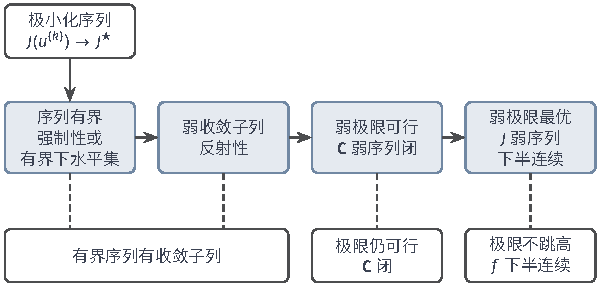
\includegraphics{figures/05-optimization/08-functional-optimization/tikz/func-direct-gates/figure.pdf}
  \caption{直接法的四步。上排蓝框是函数空间中的要求，每一步下方的白框是有限维的对应要求，有限维中有界序列必有收敛子列，所以前两步合成一个要求。}
  \label{fig:func-direct-gates}
\end{BookInlineFigure}

\begin{theorem}[直接法]
\label{thm:func-direct-method}
设$X$是实反射Banach空间，$\bm{C}\subseteq X$非空且弱序列闭，$J:\bm{C}\to\mathbb{R}\cup\{+\infty\}$弱序列下半连续。若存在实数$a$，使下水平集
\begin{equation}
 \bm{S}_a=\{u\in\bm{C}:J(u)\leq a\}
 \label{eq:func-sublevel}
\end{equation}
非空且有界，则$J^\star$是有限实数，且问题~\eqref{eq:func-problem}有最优解。
\end{theorem}

\begin{proof}
由$\bm{S}_a$非空，有$J^\star\leq a$。若$J^\star=a$，$\bm{S}_a$中的任一点已是最优解。下设$J^\star<a$，取$\bm{C}$中的序列$u^{(k)}$，使$J(u^{(k)})$递减到$J^\star$，并使各项都不超过$a$。这样的序列称为极小化序列，这里$J^\star$暂时可能是$-\infty$。

序列全在有界集$\bm{S}_a$中。$X$反射，所以有子列弱收敛到某个$u^\star\in X$，子列仍记作$u^{(k)}$。$\bm{C}$弱序列闭，所以$u^\star\in\bm{C}$。由弱序列下半连续性，
\[
 J(u^\star)\leq\liminf_{k\to\infty}J(u^{(k)})=J^\star.
\]
$J$不取$-\infty$，所以$J^\star$有限。又因$u^\star$可行，有$J(u^\star)\geq J^\star$，两式合起来得到$J(u^\star)=J^\star$。
\end{proof}

这种方法不写任何方程，直接对最小化序列取极限，称为\term{直接法}（direct method）。下水平集有界的最常见来源是强制性，即$\lVert u\rVert\to\infty$时$J(u)\to+\infty$。各条件的作用是：有界集把序列留住，反射性从中选出弱极限，弱序列闭保证弱极限合法，弱序列下半连续保证弱极限不比序列差。

\paragraph{怎样检查弱条件}
定义里的条件要对所有弱收敛序列验证，直接检查很困难。凸性把它们化成了容易检查的范数条件。先看可行集。

\begin{lemma}[闭凸集弱序列闭]
\label{lem:func-convex-weak-closed}
设$H$是Hilbert空间，$\bm{C}\subseteq H$是闭凸集。则$\bm{C}$弱序列闭。
\end{lemma}

\begin{proof}
设$u^{(k)}\in\bm{C}$，$u^{(k)}\rightharpoonup u$。令$p$为$u$到$\bm{C}$的最近点：到$\bm{C}$的距离的极小化序列，由平行四边形恒等式和凸性是Cauchy列，它的极限就是$p$。

任取$c\in\bm{C}$，$t\in(0,1]$，点$p+t(c-p)$在$\bm{C}$中，所以它到$u$的距离不小于$\lVert u-p\rVert_2$。展开平方，除以$t$，再令$t\to0$，得到
\[
 \langle u-p,\,c-p\rangle\leq0.
\]
取$c=u^{(k)}$，让$k\to\infty$。左端是固定向量$u-p$对$u^{(k)}-p$的读取，由弱收敛，得到
\[
 \lVert u-p\rVert^2=\langle u-p,\,u-p\rangle\leq0.
\]
所以$u=p\in\bm{C}$。
\end{proof}

几何上，证明说的是：若弱极限在$\bm{C}$之外，就有一个超平面把它和$\bm{C}$分开，而这个超平面对应的线性读取在弱收敛下是连续的，序列不可能跨过去。一般Banach空间中结论同样成立，称为Mazur定理，证明把最近点换成Hahn--Banach分离定理。

\begin{lemma}[凸与下半连续蕴含弱序列下半连续]
\label{lem:func-convex-weak-lsc}
设$\bm{C}$是Hilbert空间中的闭凸集，$J:\bm{C}\to\mathbb{R}\cup\{+\infty\}$是凸函数，且在范数下下半连续。则$J$弱序列下半连续。
\end{lemma}

\begin{proof}
对实数$a$，由$J$凸知$\bm{S}_a$是凸集，由下半连续和$\bm{C}$闭知$\bm{S}_a$是闭集，再由引理~\ref{lem:func-convex-weak-closed}，$\bm{S}_a$弱序列闭。

设$u^{(k)}\rightharpoonup u$，但$\liminf_kJ(u^{(k)})<J(u)$。取实数$a$严格介于两者之间，则有子列落在$\bm{S}_a$中。它的弱极限$u$也在$\bm{S}_a$中，即$J(u)\leq a$，与$a<J(u)$矛盾。
\end{proof}

回到式~\eqref{eq:func-energy}。可行集~\eqref{eq:func-feasible}是由两个连续线性条件给出的闭仿射集，是闭凸集；由式~\eqref{eq:func-point-bound}，端点读取在$H^1$中连续。$E=\frac12\lVert u\rVert_{H^1}^2$是凸的连续函数，下水平集都有界。定理~\ref{thm:func-direct-method}的条件全部满足，所以$E$的极小点存在。

\paragraph{积分目标的存在定理}
下面的结论把上述检查做成一个可以直接使用的形式。它把密度分成导数部分和函数值部分，两部分起的作用不同。

\begin{theorem}[可分离密度的存在性]
\label{thm:func-tonelli}
设$G:\mathbb{R}\to\mathbb{R}$是凸的连续函数，并存在$c>0$和$d\geq0$使$G(p)\geq cp^2-d$。设$V:[0,1]\times\mathbb{R}\to\mathbb{R}$连续且下有界。对给定的实数$\alpha,\beta$，在
\begin{equation}
 \bm{C}=\bigl\{u\in H^1(0,1):u(0)=\alpha,\ u(1)=\beta\bigr\}
 \label{eq:func-separable-feasible}
\end{equation}
上，目标
\begin{equation}
 J(u)=\int_0^1\Bigl(G\bigl(u'(x)\bigr)+V\bigl(x,u(x)\bigr)\Bigr)\,\mathrm{d}x
 \label{eq:func-separable}
\end{equation}
有极小点。
\end{theorem}

\begin{proof}
\emph{有界下水平集。}线性函数$u_0$过两个端点，$J(u_0)$有限；取$a=J(u_0)$。设$J(u)\leq a$，$V\geq-d'$，由增长条件，
\[
 c\lVert u'\rVert_2^2\leq a+d+d'.
\]
$u-u_0\in H^1_0(0,1)$，由Poincaré不等式，$\lVert u-u_0\rVert_2\leq\lVert u'-u_0'\rVert_2$。所以$\bm{S}_a$在$H^1$中有界。

\emph{可行集。}$\bm{C}$是闭仿射集，由引理~\ref{lem:func-convex-weak-closed}，它弱序列闭。

\emph{弱序列下半连续。}设$u^{(k)}\rightharpoonup u$于$H^1$，取子列使$J(u^{(k)})$趋于下极限，不妨设下极限有限。弱收敛序列有界，再由连续代表的等式和Cauchy--Schwarz不等式，
\[
 \lvert u^{(k)}(x)-u^{(k)}(y)\rvert\leq\lvert x-y\rvert^{1/2}\lVert u^{(k)\prime}\rVert_2.
\]
所以$u^{(k)}$一致有界且等度连续。由Arzelà--Ascoli定理，再取子列，它在$[0,1]$上一致收敛，极限必为$u$。$V$在紧集上一致连续，于是
\[
 \int_0^1V(x,u^{(k)})\,\mathrm{d}x\to\int_0^1V(x,u)\,\mathrm{d}x.
\]

对每个$g\in L^2$，$v\mapsto\int_0^1gv'\,\mathrm{d}x$是$H^1$上的连续线性泛函，所以$u^{(k)\prime}\rightharpoonup u'$于$L^2$。泛函$w\mapsto\int_0^1G(w)\,\mathrm{d}x$在$L^2$上是凸的。它也下半连续：范数收敛序列有几乎处处收敛的子列，$G+d\geq0$，对其用Fatou引理即可。由引理~\ref{lem:func-convex-weak-lsc}，
\[
 \int_0^1G(u')\,\mathrm{d}x\leq\liminf_{k\to\infty}\int_0^1G(u^{(k)\prime})\,\mathrm{d}x.
\]
两部分相加即得式~\eqref{eq:func-weak-lsc}，再由定理~\ref{thm:func-direct-method}得到结论。
\end{proof}

证明展示了分工。函数值$u^{(k)}$因为一维的紧嵌入而一致收敛，所以$V$不需要任何凸性。导数$u^{(k)\prime}$只有弱收敛，所以$G$必须对$p$是凸的。$E$的$G=\frac12p^2$，$V=\frac12s^2$，满足定理。

\paragraph{第一关失败：序列没有界，或者没有弱极限}
下面逐条去掉条件。第一个例子去掉强制性。考虑区间$[-1,1]$上的目标
\[
 J(u)=\int_{-1}^1x^2u'(x)^2\,\mathrm{d}x,\qquad u(-1)=-1,\ u(1)=1.
\]
权函数$x^2$在原点为零，那里的导数几乎不被惩罚。取图~\ref{fig:func-fail-bounded}(a)的折线$u^{(k)}(x)=\max\{-1,\min\{1,kx\}\}$，导数只在$\lvert x\rvert<1/k$上非零，等于$k$。代入得到
\[
 J(u^{(k)})=\int_{-1/k}^{1/k}x^2k^2\,\mathrm{d}x=\frac{2}{3k}\to0.
\]

所以$J^\star=0$。若有$u\in H^1(-1,1)$使$J(u)=0$，则$u'=0$几乎处处，$u$是常数，这与两端的值$-1,1$矛盾，极小点不存在。此时导数的长度$\lVert u^{(k)\prime}\rVert_2^2=2k$趋于无穷，序列在$H^1$中无界，$J$不强制。序列想要趋向的跳跃函数也不在$H^1$中。

\begin{BookInlineFigure}
  \centering
  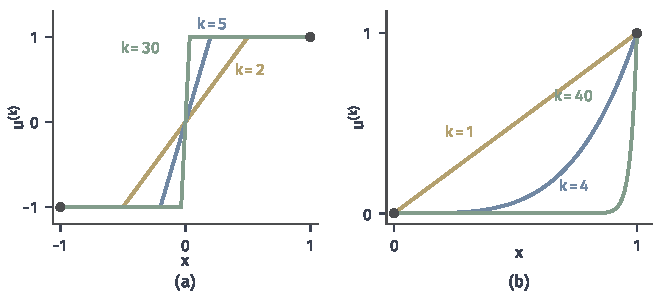
\includegraphics[width=112mm]{figures/05-optimization/08-functional-optimization/matplotlib/func-fail-bounded/figure.pdf}
  \caption{第一关的两种失败，灰点是固定端点。(a)$\int_{-1}^1x^2u'^2\,\mathrm{d}x$的极小化序列$u^{(k)}=\max\{-1,\min\{1,kx\}\}$，目标值$2/(3k)$趋于零，导数的长度趋于无穷。(b)$\int_0^1(\lvert u'\rvert+u^2)\,\mathrm{d}x$的极小化序列$u^{(k)}=x^k$，$W^{1,1}$范数有界，所有质量向$x=1$处的跳跃集中。}
  \label{fig:func-fail-bounded}
\end{BookInlineFigure}

第二个例子去掉反射性。在$W^{1,1}(0,1)$上取端点条件$u(0)=0$、$u(1)=1$，目标
\[
 J(u)=\int_0^1\bigl(\lvert u'(x)\rvert+u(x)^2\bigr)\,\mathrm{d}x.
\]
曲线从$0$升到$1$，导数绝对值的积分不小于总上升量：
\[
 \int_0^1\lvert u'\rvert\,\mathrm{d}x\geq\lvert u(1)-u(0)\rvert=1.
\]
所以$J\geq1$。取图~\ref{fig:func-fail-bounded}(b)的$u^{(k)}=x^k$，它单调上升，所以
\[
 J(u^{(k)})=1+\frac{1}{2k+1}\to1.
\]

因此$J^\star=1$。若$J(u)=1$，则$\int_0^1u^2\,\mathrm{d}x=0$，$u$恒为零，与$u(1)=1$矛盾，极小点不存在。这次序列有界，它的$W^{1,1}$范数满足
\[
 \lVert u^{(k)}\rVert_1+\lVert u^{(k)\prime}\rVert_1\leq2.
\]
但它没有弱收敛子列。若有，弱极限几乎处处等于序列的逐点极限$0$，而端点读取在$W^{1,1}$中连续，弱极限在$x=1$处又应等于$1$。把平方积分的$\lvert u'\rvert^2$换成$\lvert u'\rvert$，反射性就失去了，定理~\ref{thm:func-tonelli}中$cp^2$的增长条件正是在防止这种情况。

\paragraph{第二关失败：弱极限不可行}
闭集未必弱序列闭。取$\bm{C}$为$L^2(0,1)$中的单位球面，目标$J(u)=\int_0^1x\,u(x)^2\,\mathrm{d}x$。这相当于分配总量为$1$的质量，放在$x$处的代价是$x$，质量当然想挤到原点。取$u^{(k)}=\sqrt{k}\,\mathbf{1}_{[0,1/k]}$，见图~\ref{fig:func-fail-sphere}，得到
\[
 \lVert u^{(k)}\rVert_2=1,\qquad J(u^{(k)})=k\int_0^{1/k}x\,\mathrm{d}x=\frac{1}{2k}\to0.
\]

\begin{BookInlineFigure}
  \centering
  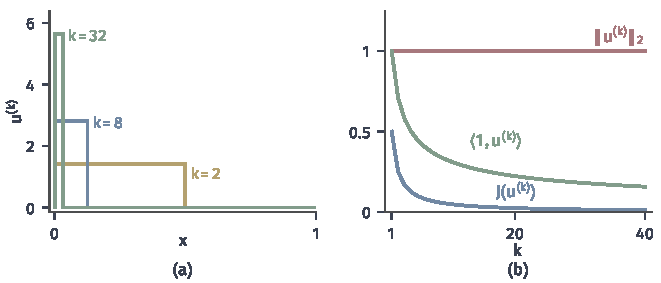
\includegraphics[width=112mm]{figures/05-optimization/08-functional-optimization/matplotlib/func-fail-sphere/figure.pdf}
  \caption{第二关的失败：单位球面不弱序列闭。(a)$u^{(k)}=\sqrt{k}\,\mathbf{1}_{[0,1/k]}$越来越高、越来越窄。(b)红线是不变的长度，绿线是读取$\langle1,u^{(k)}\rangle=k^{-1/2}$，蓝线是目标值$1/(2k)$。}
  \label{fig:func-fail-sphere}
\end{BookInlineFigure}

$J(u)=0$要求$u=0$几乎处处，但零函数不在球面上，所以极小点不存在。对任意$g\in L^2$，由Cauchy--Schwarz不等式，
\[
 \lvert\langle g,u^{(k)}\rangle\rvert\leq\lVert g\rVert_{L^2(0,1/k)}\to0.
\]
所以$u^{(k)}\rightharpoonup0$。球面上的序列弱收敛到球心，弱极限离开了可行集。在有限维中球面是紧集，这个现象不会发生。把可行集放大成单位闭球，它是闭凸集，极小点$u=0$立即存在。

\paragraph{第三关失败：弱极限比序列差}
最后去掉对导数的凸性。在$H^1(0,1)$上考虑
\begin{equation}
 J(u)=\int_0^1\Bigl(\bigl(u'(x)^2-1\bigr)^2+u(x)^2\Bigr)\,\mathrm{d}x,\qquad u(0)=u(1)=0,
 \label{eq:func-bolza}
\end{equation}
其中$u'\notin L^4$时$J$取$+\infty$。第一项希望斜率是$\pm1$，第二项希望$u$接近零。取图~\ref{fig:func-bolza-zigzag}(a)的锯齿$z_k$：$k$个相同的齿，斜率$\pm1$，高度$1/(2k)$。第一项为零，第二项每个齿贡献$\frac{2}{3}(2k)^{-3}$，总计
\[
 J(z_k)=k\cdot\frac23\cdot\frac{1}{8k^3}=\frac{1}{12k^2}\to0.
\]

\begin{BookInlineFigure}
  \centering
  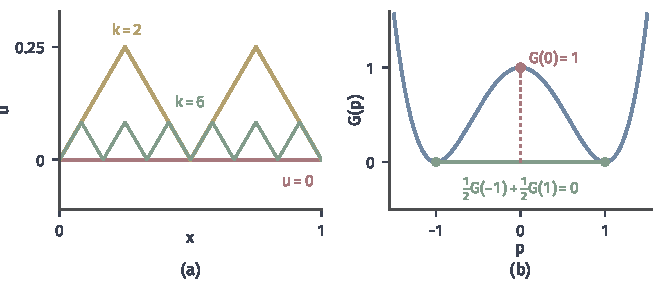
\includegraphics[width=112mm]{figures/05-optimization/08-functional-optimization/matplotlib/func-bolza-zigzag/figure.pdf}
  \caption{第三关的失败。(a)目标~\eqref{eq:func-bolza}的锯齿极小化序列，黄色$k=2$，绿色$k=6$，红线是弱极限$u=0$。(b)导数部分的密度$G(p)=(p^2-1)^2$：斜率$\pm1$各占一半时，平均代价是绿线上的$0$，而平均斜率$0$自身的代价是红点$1$。}
  \label{fig:func-bolza-zigzag}
\end{BookInlineFigure}

所以$J^\star=0$。$J(u)=0$要求$u=0$，同时要求$\lvert u'\rvert=1$几乎处处，二者矛盾，极小点不存在。序列在$H^1$中有界，并且$z_k\rightharpoonup0$，弱极限$0$是可行的，但$J(0)=1$。弱极限比序列差了整整一个单位，式~\eqref{eq:func-weak-lsc}不成立。

机制在图~\ref{fig:func-bolza-zigzag}(b)。弱收敛只记住了斜率的局部平均，而锯齿的平均斜率是$0$。$G$在$\pm1$处为零，而在两者的平均$0$处等于$1$，这就是$G$非凸。若$G$是凸的，Jensen不等式给出“平均的代价不超过代价的平均”，弱极限就不会变差。

\paragraph{驻定不能代替存在}
还有一种常见的想法：写出令导数为零的方程，解出来就是答案。下面的例子说明，这样做既不能证明解存在，得到的候选也未必是解。在$\bm{V}=H^1_0(0,1)$上取实数$\rho$，考虑
\begin{equation}
 J_\rho(u)=\int_0^1\Bigl(\frac12u'(x)^2-\frac{\rho}{2}u(x)^2\Bigr)\,\mathrm{d}x.
 \label{eq:func-rho}
\end{equation}
沿任何一条过原点的直线都有$J_\rho(t\eta)=t^2J_\rho(\eta)$，这是$t$的一元二次函数，在$t=0$处导数为零。所以$u=0$沿每个方向都是平的，它满足任何合理的驻定条件。

取方向$\eta(x)=\sin\pi x$。由$\int_0^1\eta'^2\,\mathrm{d}x=\pi^2/2$，$\int_0^1\eta^2\,\mathrm{d}x=1/2$，得到
\[
 J_\rho(t\sin\pi x)=\frac{t^2}{4}(\pi^2-\rho).
\]
图~\ref{fig:func-stationary-no-min}画了三种情形。$\rho>\pi^2$时，沿这个方向目标趋于$-\infty$，$J_\rho^\star=-\infty$，极小点不存在，而$u=0$仍然驻定。

\begin{BookInlineFigure}
  \centering
  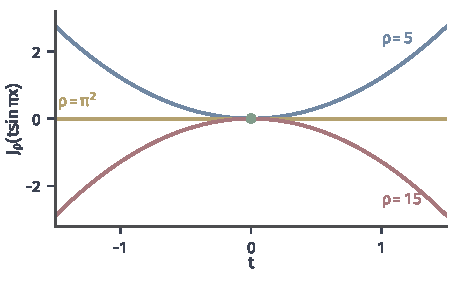
\includegraphics[width=78mm]{figures/05-optimization/08-functional-optimization/matplotlib/func-stationary-no-min/figure.pdf}
  \caption{目标~\eqref{eq:func-rho}沿$t\sin\pi x$的取值。绿点$t=0$在三种情形下都驻定。$\rho=5$时是开口向上的抛物线，$\rho=\pi^2$时恒为零，$\rho=15$时向下，目标无下界。}
  \label{fig:func-stationary-no-min}
\end{BookInlineFigure}

这个$J_\rho$对每个$\rho$都弱序列下半连续：$\int u'^2$部分是凸的，$\int u^2$部分在弱收敛下连续。失败的只是下水平集的有界性。“若极小点存在，则它满足驻定方程”是一个条件命题，它的前提要靠本节的论证另行建立。
